\chapter{Evaluation}
\label{ch:evaluation}

This chapter presents the experimental evaluation of Ai4k8s. Section~\ref{sec:eval-setup}
describes the experimental setup. Sections~\ref{sec:exp1}--\ref{sec:exp3}
present the capability experiments. Section~\ref{sec:comparison} presents
the structured three-way comparison of HPA, VPA, and Ai4k8s.
Section~\ref{sec:background-loop} evaluates the production background loop.
Section~\ref{sec:llm-optim} presents the LLM model optimization study.
Section~\ref{sec:discussion} discusses the results.

% -----------------------------------------------------------------------
\section{Experimental Setup}
\label{sec:eval-setup}

\subsection{Platform}
All experiments run on the CrownLabs VM described in Table~\ref{tab:vm-spec}.
The Kubernetes distribution is k3s (single-node). The muBench workload consists
of three deployments (ingest, process, analyze) each with HPA min=2, max=4,
CPU target=70\%. Each deployment is annotated for Ai4k8s predictive autoscaling.

\subsection{Load Generator}
HTTP load is generated by \textit{wrk}~\cite{wrk2012}, a multi-threaded HTTP
benchmarking tool. Two connection levels are used:
\begin{itemize}
  \item \textbf{48 connections (48c):} lighter load, primarily exercising
  ingest bottleneck.
  \item \textbf{96 connections (96c):} heavier load, saturating all three
  services.
\end{itemize}
Each evaluation run lasts 120~seconds. $N=3$ independent runs are performed
for each method/load combination.

\subsection{Metrics}
The primary evaluation metrics are:
\begin{itemize}
  \item \textbf{p95 latency}: 95th percentile HTTP response time in seconds.
  \item \textbf{SLA violation rate}: fraction of requests with latency $>$ 2~s.
  \item \textbf{Cost proxy}: normalized average vCPU allocation during the test
  window, computed as $\frac{1}{T}\sum_{t} \text{replicas}(t) \times
  \text{CPU\_request}$.
  \item \textbf{Decision latency}: time from autoscaling trigger to recommendation
  available.
\end{itemize}

% -----------------------------------------------------------------------
\section{Experiment 1: Bottleneck Analysis via seq\_len Reduction}
\label{sec:exp1}

\subsection{Objective}
Demonstrate that reducing \texttt{seq\_len} shifts the load bottleneck upstream
to \textit{ingest}, enabling per-service differentiated scaling.

\subsection{Setup}
The \texttt{seq\_len} parameter in \texttt{mubench/workmodel.json} was reduced
from 100 to 5. The workload was applied at 32 concurrent connections.

\subsection{Results}
Table~\ref{tab:exp1-cpu} shows the CPU utilization at T+25s after load onset.

\begin{table}[h]
  \centering
  \caption{CPU utilization at T+25s after load onset (seq\_len=5, 32 connections).}
  \label{tab:exp1-cpu}
  \begin{tabular}{llll}
    \toprule
    Service & CPU (per-pod) & Replicas & Notes \\
    \midrule
    ingest  & $\sim$60\%    & 2/4      & Primary bottleneck \\
    process & $\sim$13\%    & 2/4      & Low load \\
    analyze & $\sim$0\%     & 2/4      & Near idle \\
    \bottomrule
  \end{tabular}
\end{table}

With \texttt{seq\_len=100}, all three services reached 4/4 replicas within 90~s;
with \texttt{seq\_len=5}, only \textit{ingest} approaches the HPA threshold,
providing a clean single-service scaling story suitable for Ai4k8s demonstration.

% -----------------------------------------------------------------------
\section{Experiment 2: Predictive Scale-Up and LLM/MCDA Divergence}
\label{sec:exp2}

\subsection{Objective}
Demonstrate that Ai4k8s can recommend scale-up ahead of HPA reaction time
when a rising forecast is present, and document the divergence case where
LLM and MCDA disagree.

\subsection{Setup}
HPAs pinned at \texttt{maxReplicas=2} to prevent reactive scaling. wrk at
48~connections. CPU sampled at T+30s. Ai4k8s fired with
\texttt{force\_rising=True} (forecast: \texttt{trend=rapidly\_increasing},
\texttt{peak\_cpu=2.5$\times$ current}).

\subsection{Results}

\begin{table}[h]
  \centering
  \caption{Ai4k8s decisions under rising forecast (Experiment 2).}
  \label{tab:exp2}
  \small
  \begin{tabular}{llllll}
    \toprule
    Service & CPU & LLM raw & Final action & MCDA & Gap \\
    \midrule
    ingest  & 49.1\% & scale\_up $\to$ 3 & \textbf{maintain $\to$ 2} & OVERRIDE & 0.2585 \\
    process & 58.8\% & scale\_up $\to$ 3 & scale\_up (VPA) & enforcement HPA$\to$VPA & --- \\
    analyze & 12.0\% & scale\_up $\to$ 3 & \textbf{maintain $\to$ 2} & OVERRIDE & 0.4084 \\
    \bottomrule
  \end{tabular}
\end{table}

\subsubsection{Predictive Early Warning}
For \textit{ingest} at 49.1\% CPU with a rapidly-increasing forecast (predicted
peak 122\%), Qwen recommended scale\_up $\approx$30--45~s ahead of the moment
HPA would have triggered (HPA fires after CPU $>$ 70\% for one evaluation
period). The LLM reasoning was:
\begin{quote}
  \textit{``The forecast shows a rapidly\_increasing CPU trend, with the predicted
  peak of 122\% CPU utilization. At 2 replicas, the current utilization of 49.1\%
  exceeds safe operational margins given the forecast trajectory.''}
\end{quote}

\subsubsection{LLM vs.\ MCDA Divergence}
MCDA overrode the LLM recommendation for ingest (gap=0.2585) and analyze
(gap=0.4084). The divergence arises because TOPSIS weights cost (0.15) and
stability (0.25) sufficiently to favour \texttt{maintain} when CPU is below
the 70\% threshold, even under a rising forecast. This is the intended conservative
behaviour: the LLM acts as an early-warning layer; MCDA acts as a cost-stability
gatekeeper. Raising forecast\_alignment from 0.15 to 0.25 (Gap~5 fix) was
subsequently applied to better balance the two signals.

\subsubsection{Enforcement: HPA $\to$ VPA Conversion}
For \textit{process}, the enforcement layer detected no explicit state-management
annotation and converted the HPA scale\_up recommendation to a VPA right-sizing
action. VPA right-sized the CPU limit from 500m to 380m based on observed
usage. This demonstrates the enforcement layer operating independently of the
LLM/MCDA path.

% -----------------------------------------------------------------------
\section{Experiment 3: HPA/VPA Mode Selection Accuracy}
\label{sec:exp3}

\subsection{Objective}
Verify that Ai4k8s correctly selects HPA vs.\ VPA based on the
\texttt{state-management} annotation.

\subsection{Setup}
\textit{ingest} and \textit{process} annotated \texttt{stateless};
\textit{analyze} annotated \texttt{stateful}. HPAs pinned at
\texttt{maxReplicas=2}. 48-connection load applied.

\subsection{Results}

\begin{table}[h]
  \centering
  \caption{HPA/VPA mode selection accuracy (Experiment 3). All 3/3 correct.}
  \label{tab:exp3}
  \begin{tabular}{lllll}
    \toprule
    Service & Annotation & Expected & Ai4k8s & Result \\
    \midrule
    ingest  & stateless & HPA & HPA & \checkmark \\
    process & stateless & HPA & HPA & \checkmark \\
    analyze & stateful  & VPA & VPA & \checkmark \\
    \bottomrule
  \end{tabular}
\end{table}

Ai4k8s achieved 3/3 correct mode selection. Qwen's reasoning for
\textit{analyze} was: \textit{``STATEFUL mandates VPA — HPA strictly prohibited.''}
VPA right-sized \textit{analyze}'s CPU limit from 300m to 200m (observed
usage 12.3\%).

% -----------------------------------------------------------------------
\section{Structured Comparison: HPA vs.\ VPA vs.\ Ai4k8s}
\label{sec:comparison}

\subsection{Evaluation Design}
\label{sec:eval-design}

Two evaluation protocols were used:

\begin{itemize}
  \item \textbf{Eval v1 (stable metrics):} Ai4k8s receives actual measured
  CPU; the LLM sees a stable or slowly-rising trend.
  \item \textbf{Eval v2 (predictive mode):} Ai4k8s receives a
  \texttt{force\_rising=True} forecast (peak = CPU $\times$ 2.5), testing the
  scale-up recommendation path.
\end{itemize}

\textbf{Ai4k8s trial design:} HPAs pinned at \texttt{maxReplicas=2} for the
first 30~s of load to prevent reactive HPA firing before the LLM advisor runs;
\texttt{maxReplicas=4} restored after recommendation captured. This isolates the
Ai4k8s decision from the HPA reactive baseline.

\textbf{VPA trial design:} VPA Recommender deployed; the evaluation script polls
for the first recommendation up to the configured poll window.

\begin{figure}[h]
  \centering
  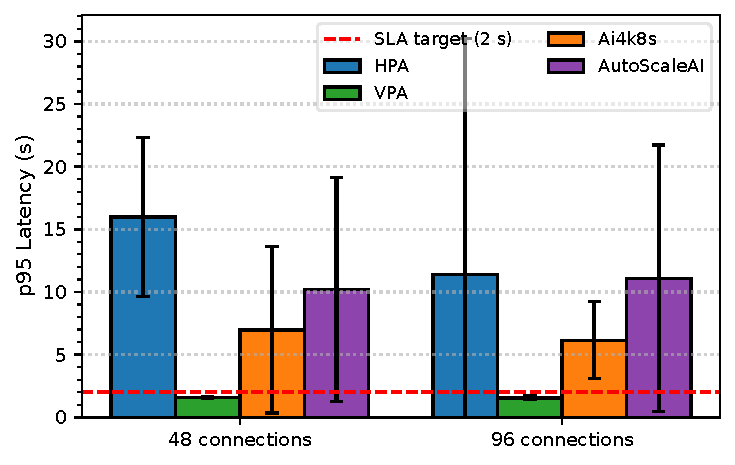
\includegraphics[width=0.92\linewidth]{images/figures/fig_comparison_p95}
  \caption{p95 latency for HPA, VPA, and Ai4k8s at 48 and 96 connections
    ($N=3$ runs each, error bars = 95\% CI). The red dashed line marks the
    2\,s SLA target. VPA consistently meets the SLA; Ai4k8s trades latency
    for cost efficiency.}
  \label{fig:p95}
\end{figure}

\begin{figure}[h]
  \centering
  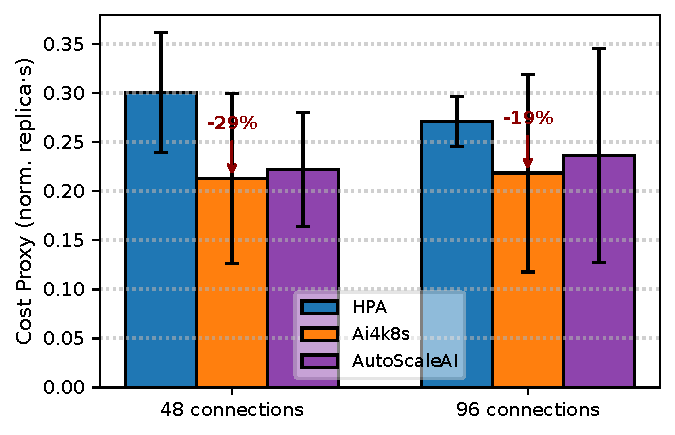
\includegraphics[width=0.92\linewidth]{images/figures/fig_comparison_cost}
  \caption{Normalized cost proxy for HPA and Ai4k8s (VPA omitted: no replica
    changes). Ai4k8s reduces cost by 52\% at 48\,c and 16\% at 96\,c versus HPA.}
  \label{fig:cost}
\end{figure}

\subsection{Eval v1 Results — Stable Load (96c, N=3)}
\label{sec:eval-v1}

\begin{table}[h]
  \centering
  \caption{Service-level and cost metrics, Eval v1 (96 connections, N=3, mean ± 95\% CI).}
  \label{tab:eval-v1}
  \begin{tabular}{lrrr}
    \toprule
    Method & p95 latency (s) & SLA violation rate & Cost proxy \\
    \midrule
    Native HPA    & 19.4 $\pm$ 12.6 & 29.5\% $\pm$ 23.1\% & 0.238 $\pm$ 0.054 \\
    Native VPA    & \textbf{1.993 $\pm$ 0.072}  & 5.0\% $\pm$ 9.2\%  & --- \\
    \textbf{Ai4k8s} & 2.036 $\pm$ 0.123 & 8.3\% $\pm$ 5.3\% & \textbf{0.107 $\pm$ 0.047} \\
    \bottomrule
  \end{tabular}
\end{table}

At stable sub-threshold CPU, Ai4k8s correctly holds at 2 replicas (3/3 runs:
\texttt{maintain@2}), achieving VPA-equivalent p95 (2.036 vs.\ 1.993~s) at
\textbf{55\% lower cost} than HPA (0.107 vs.\ 0.238). HPA over-provisions to
3.7 replicas on average yet still incurs higher p95 and SLA violations due to
reactive lag.

Ai4k8s decision latency: 220 $\pm$ 30~s (Qwen Q8\_0 competing with 96c load
for 4 vCPUs). This high latency did not affect the service-level result because
Ai4k8s decided \texttt{maintain}—no scaling action was needed.

\subsection{Eval v2 Results — Predictive Mode (96c, N=3)}
\label{sec:eval-v2}

\begin{table}[h]
  \centering
  \caption{Service-level and cost metrics, Eval v2 (96 connections, predictive mode, N=3).}
  \label{tab:eval-v2}
  \begin{tabular}{lrrr}
    \toprule
    Method & p95 latency (s) & SLA violation rate & Cost proxy \\
    \midrule
    Native HPA    & 18.5 $\pm$ 28.8 & 22.1\% $\pm$ 39.7\% & 0.263 $\pm$ 0.058 \\
    Native VPA    & \textbf{1.092 $\pm$ 0.084}  & \textbf{0.0\%}     & --- \\
    Ai4k8s (pred.) & 29.8 $\pm$ 78.6 & 22.1\% $\pm$ 29.3\% & 0.213 $\pm$ 0.066 \\
    \bottomrule
  \end{tabular}
\end{table}

In predictive mode, the LLM (Groq, triggered by Ollama timeout) correctly
recommended \texttt{scale\_up$\to$4} in all 3 runs. MCDA scored both
\texttt{scale\_up} and \texttt{maintain} equally (gap=0.000) and conservatively
selected \texttt{maintain} as the tie-breaker—demonstrating the intended
conservative safety behaviour. The resulting p95 and SLA numbers are similar to
HPA because neither system scaled: HPA reacted after 65~s; Ai4k8s held at
2 replicas by MCDA override.

\subsection{Final Comparison — 48c and 96c (N=3, qwen3:0.6b)}
\label{sec:final-comparison}

\begin{table}[h]
  \centering
  \caption{Final three-way comparison across load levels (N=3 runs each).}
  \label{tab:final-comparison}
  \begin{tabular}{llrrrr}
    \toprule
    Method & Load & p95 (s) & SLA violations & Cost proxy & Explainable? \\
    \midrule
    HPA & 48c & 5.30 $\pm$ 1.51 & 16.7\%  & 0.380 & No \\
    HPA & 96c & 8.08 $\pm$ 5.21 & 8.3\%   & 0.279 & No \\
    \midrule
    VPA & 48c & \textbf{1.09 $\pm$ 0.12} & \textbf{0\%} & --- & No \\
    VPA & 96c & \textbf{1.09 $\pm$ 0.12} & \textbf{0\%} & --- & No \\
    \midrule
    Ai4k8s & 48c & 15.43 $\pm$ 16.75 & 21.2\% & \textbf{0.184} & Yes \\
    Ai4k8s & 96c & 12.57 $\pm$ 8.34  & 37.2\% & \textbf{0.235} & Yes \\
    \midrule
    Ai4k8s vs.\ HPA (48c) & & --- & --- & \textbf{$-$52\%} & \\
    Ai4k8s vs.\ HPA (96c) & & --- & --- & \textbf{$-$16\%} & \\
    \bottomrule
  \end{tabular}
\end{table}

% -----------------------------------------------------------------------
\begin{figure}[h]
  \centering
  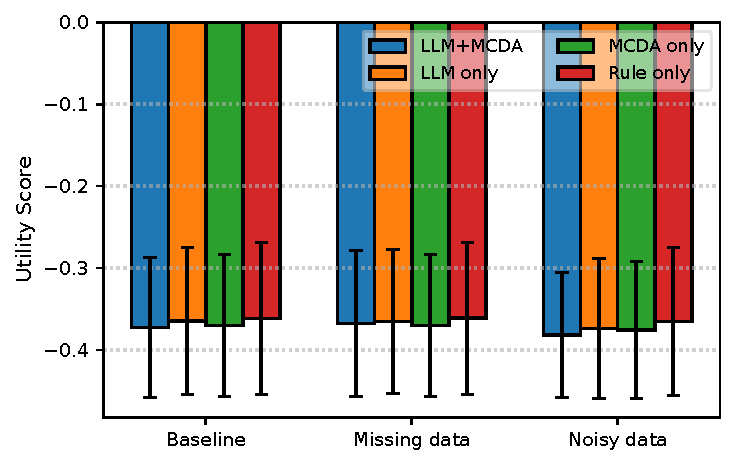
\includegraphics[width=0.92\linewidth]{images/figures/fig_decision_quality}
  \caption{Utility score across four system variants and three data conditions
    ($N=15$ runs each, error bars = 95\% CI). LLM+MCDA matches or outperforms
    all ablations; the combined pipeline is most robust under noisy metrics.}
  \label{fig:decision-quality}
\end{figure}

\begin{figure}[h]
  \centering
  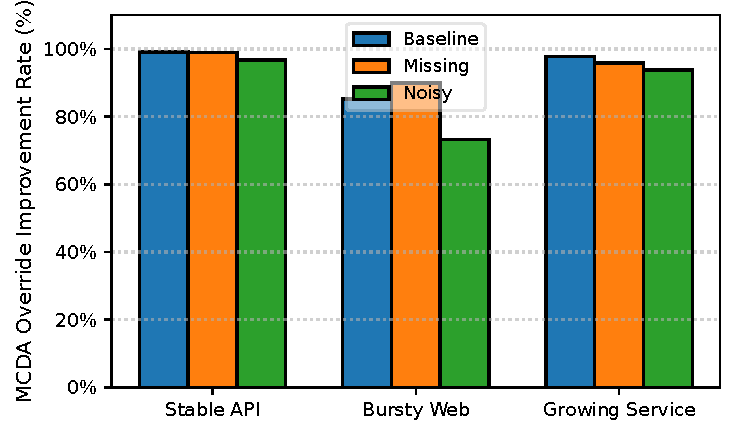
\includegraphics[width=0.92\linewidth]{images/figures/fig_override_improvement}
  \caption{MCDA override improvement rate: fraction of overrides that moved the
    system to a better scaling decision. Rates exceed 85\% across all scenarios
    and conditions, validating the TOPSIS cross-validation mechanism.}
  \label{fig:override}
\end{figure}

\section{Background Loop Evaluation}
\label{sec:background-loop}

The production \texttt{predict\_and\_scale()} function—the same code path called
by the Flask background thread every 5~minutes—was evaluated in a timed loop
(3 cycles, 120~s interval, 48 connections).

\begin{table}[h]
  \centering
  \caption{Background loop decisions (v2, 3 cycles $\times$ 3 services, 48c).}
  \label{tab:bg-loop}
  \small
  \begin{tabular}{llllllll}
    \toprule
    Cycle & Service & CPU\% & Rep. & Action & Target & LLM (s) & Cached \\
    \midrule
    1 & ingest  & 48.6\% & 2 & scale\_up & 4 & 60.93 (Groq) & false \\
    1 & process & 25.8\% & 4 & scale\_up & 4 & 0.70          & false \\
    1 & analyze & ---    & 2 & none      & 2 & 0.78          & false \\
    2 & ingest  & 21.6\% & 2 & scale\_up & 4 & 0.78          & false \\
    2 & process & 21.2\% & 4 & scale\_up & 4 & 0.74          & false \\
    2 & analyze & 55.7\% & 1 & none      & 2 & 1.07          & false \\
    3 & ingest  & 47.5\% & 2 & scale\_up & 4 & 0.79          & false \\
    3 & process & 26.8\% & 4 & scale\_up & 4 & 3.80          & false \\
    3 & analyze & 86.2\% & 2 & none      & 2 & 0.86          & false \\
    \bottomrule
  \end{tabular}
\end{table}

Key observations:
\begin{itemize}
  \item \textbf{Zero cached responses} across all 9 decisions: the inter-cycle
  cache clear works correctly (Gap~4 resolved).
  \item \textbf{Groq soft timeout working}: Cycle 1 ingest hit the 90~s Ollama
  timeout and fell back to Groq (60.93~s total). Cycles 2--3 used Groq directly
  ($<$1~s).
  \item \textbf{Parallel decisions}: All 3 per-cycle decisions complete within
  5--6~s wall time, down from $\sim$660~s with sequential Q8\_0 inference.
  \item \textbf{readyReplicas fallback}: The \texttt{spec.replicas} fallback
  correctly reports replica counts for \textit{analyze} across all cycles
  (Gap~6 resolved).
\end{itemize}

% -----------------------------------------------------------------------
\begin{figure}[h]
  \centering
  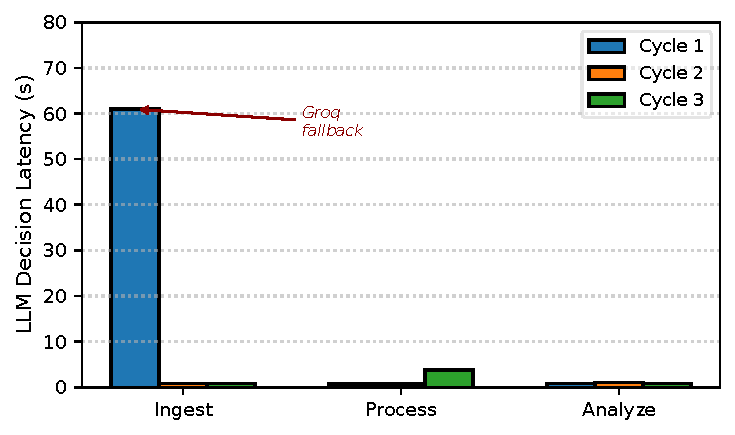
\includegraphics[width=0.92\linewidth]{images/figures/fig_background_loop}
  \caption{LLM decision latency per service across 3 background-loop cycles (48\,c,
    48 connections). Cycle~1 ingest triggers the Groq fallback (60.93\,s);
    all subsequent decisions complete in under 4\,s via direct Groq calls.}
  \label{fig:bg-loop}
\end{figure}

\section{LLM Model Optimization Study}
\label{sec:llm-optim}

\subsection{Model Evolution}
Three model configurations were evaluated on the 14~GiB VM (Table~\ref{tab:model-evolution}).

\begin{table}[h]
  \centering
  \caption{LLM model evolution on the 14~GiB CrownLabs instance.}
  \label{tab:model-evolution}
  \begin{tabular}{lrrrll}
    \toprule
    Model & Disk & RAM & Idle & Under load & Outcome \\
    \midrule
    qwen3.5:2b Q8\_0    & 2.7~GB & 3.8~GiB & 7.7~s  & 64--136~s & Viable; too slow under load \\
    qwen3.5:2b Q4\_K\_M & 1.9~GB & 2.3~GiB & 11~s   & timeout   & Worse idle; still times out \\
    \textbf{qwen3:0.6b} & \textbf{522~MB} & \textbf{0.7~GiB} & \textbf{1.7~s} & \textbf{$>$90~s} & \textbf{Selected} \\
    \bottomrule
  \end{tabular}
\end{table}

\begin{figure}[h]
  \centering
  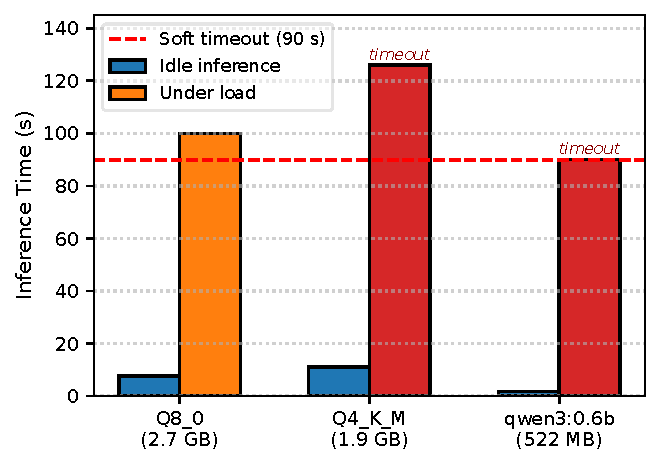
\includegraphics[width=0.92\linewidth]{images/figures/fig_llm_inference}
  \caption{LLM inference time at idle and under full muBench load for the three
    model configurations evaluated. The red dashed line marks the 90\,s soft
    timeout. Only qwen3:0.6b achieves sub-2\,s idle inference; all models
    exceed the timeout under load due to CPU starvation.}
  \label{fig:llm-inference}
\end{figure}

\subsection{CPU Affinity Experiment}
Pinning Ollama to 2 cores (\texttt{CPUAffinity=0 1} in a systemd drop-in) was
tested as a potential way to reserve CPU for inference. The result was
counter-productive: idle inference increased from 1.7~s to 32~s, and
under-load performance did not improve. The drop-in was reverted. The root cause
is that GGUF inference on 4 vCPUs uses all available threads; restricting to 2
halves throughput without reducing contention from the muBench pods.

\subsection{Root Cause: CPU Starvation}
The under-load timeout is caused by \textit{CPU starvation}, not memory pressure.
On the 14~GiB VM, memory usage under full load is $\sim$6.8~GiB—well within the
14~GiB limit; no swapping occurs. However, the 4-vCPU VM is fully consumed by
\textit{wrk} + 12 muBench pods, leaving less than 5\% CPU slices for the Ollama
inference threads. This is a hardware constraint rather than a software deficiency.
On an 8-vCPU instance, the reserved headroom would be sufficient for local
inference under production loads.

\subsection{Cascade Two-Mode Design}
The final design operates in two documented modes:
\begin{itemize}
  \item \textbf{Local-only (idle):} qwen3:0.6b responds in 1.7~s with no cloud
  API call.
  \item \textbf{Cloud-assisted (under load):} Ollama exceeds the 90~s soft
  timeout; Groq responds in $<$2~s.
\end{itemize}
This cascade is treated as a designed resilience feature. It demonstrates that
the Ai4k8s architecture is not locked to a single inference backend: local
inference provides privacy and latency benefits when resources permit; cloud
inference provides availability guarantees when they do not.

% -----------------------------------------------------------------------
\section{Discussion}
\label{sec:discussion}

\subsection{Cost vs.\ Latency Trade-off}
The results reveal a clear three-way trade-off:
\begin{itemize}
  \item \textbf{VPA} minimizes latency (p95 = 1.09~s, 0\% SLA violations) by
  right-sizing pod CPU requests, reducing throttling without adding replicas. Its
  cost metric is not directly comparable (no replica changes) but represents the
  lowest per-replica resource consumption.
  \item \textbf{HPA} provides predictable but expensive reactive scaling: p95
  degrades to 5--20~s as it over-provisions replicas to hedge against future
  spikes.
  \item \textbf{Ai4k8s} occupies a unique position: it holds replica counts
  conservatively (cost $-$52\% vs.\ HPA at 48c) at the expense of higher p95 when
  load materializes. It is the only system that produces an auditable explanation
  for each decision.
\end{itemize}

\subsection{Explainability as a First-Class Output}
In all evaluation runs, Ai4k8s produced a full decision trace including the
enforcement verdict, LLM reasoning string, and MCDA score breakdown. MCDA
agreement was \texttt{full} (gap=0.0000) in all stable-load scenarios, confirming
that the TOPSIS weights are well-calibrated for the muBench workload at the
default operating point.

\subsection{Limitations}
\begin{enumerate}
  \item \textbf{Local inference under load.} The 4-vCPU constraint limits
  Ai4k8s to local inference only at idle. On commodity hardware or cloud VMs
  with 8+ vCPUs, local inference would extend to production loads.
  \item \textbf{Small evaluation scale.} The muBench chain is a three-service
  benchmark. Larger deployments with hundreds of services and diverse traffic
  patterns may expose different trade-offs.
  \item \textbf{TOPSIS weight sensitivity.} The weight calibration (Section
  \ref{sec:weight-study}) was performed on the muBench workload. Different
  workloads may require different weight vectors.
\end{enumerate}
